\subsubsection{02.03.2016}
\textit{\textbf{Time frame:}} 19:00-21:00 

Today it was found the optimal principle of building the lifting mechanism (figure \ref{Elevator4.5}). It was found out that if two slats are placed at the angle of $90^circ$, they form the most firm construction with a good resistance against bend.

\begin{figure}[H]
	\begin{minipage}[h]{1\linewidth}
		\center{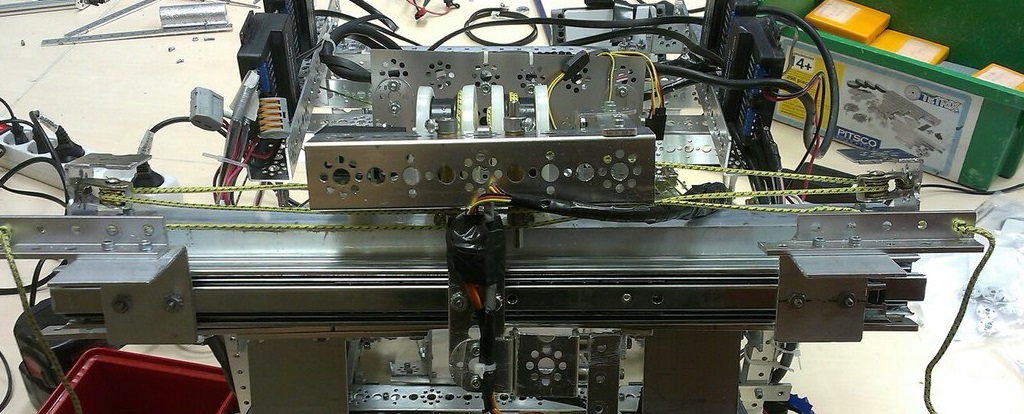
\includegraphics[scale=0.2]{3Engineering/5Team_meetings/days_of_meetings/2016.03.02/images/01}}
		\caption{Optimal construction}
		\label{Elevator4.5}
	\end{minipage}
\end{figure}
